Lst. \ref{lst:ex8} shows the modification to the pseudo-code of alpha-beta to introduce a harder pruning, paying with returning the non-best results, worsened possibly by the factor $\epsilon$.

\begin{lstlisting}[language=python, label={lst:ex8}, caption={Modified code: the changes are in lines 110-11 and 21-22.}]
    alphaBeta(state):
        return maxValue(state, -INFINITY, INFINITY, 0)

    maxValue(state, alpha, beta, depth):
        if cutoffTest(state, depth):
            return utility (state)
        value = -INFINITY
        for successor in state.getSuccessors():
            value= max(value, minValue(successor, alpha, beta, depth + 1))
            if value + eps >= beta: # modified
                return value  + eps # modified
            alpha= max(alpha, value).
        return value

    minValue(state, alpha, beta, depth):
        if cutoffTest(state, depth):
            return utility(state)
        value = INFINITY
        for successor in state.getSuccessors():
            value=min(value, maxValue(successor, alpha, beta, depth + 1)
            if value - eps <= alpha: # modified
                return value - eps # modified
            beta min(beta, value)
        return value
\end{lstlisting}

The new algorithm returns a result different from the minimax in the case shown in Fig. \ref{fig:8_b}. In this case, alpha-beta prunes away the sub-tree after edge $a3$, and returns $a1$ with the optimal minimax value of 40. Minimax, on the other hand, returns $a3$ with optimal minimax value of 42.
\begin{figure}[h]
    \centering
    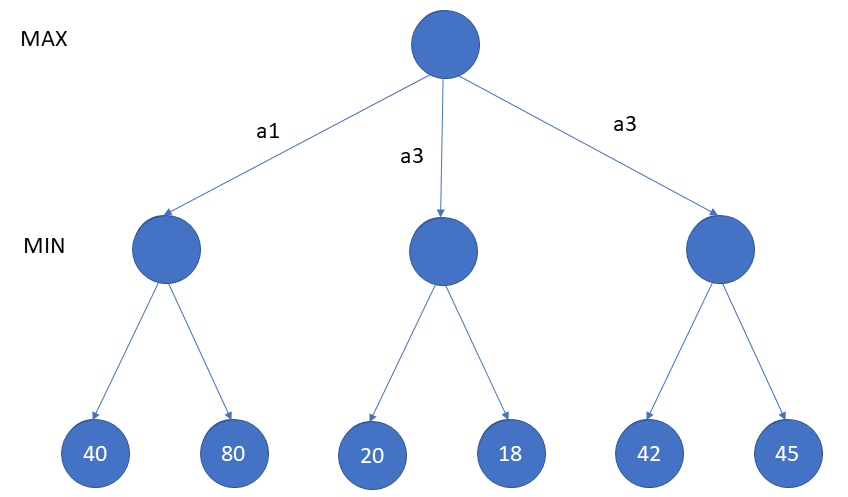
\includegraphics[width=1\linewidth]{8_b}
    \caption{With $\epsilon = 2.5$, $42 -\epsilon = 39.5 < 40$ and therefore alpha-beta modified prunes away the sub-tree child of edge $a3$.}
    \label{fig:8_b}
\end{figure}
